\documentclass{article}
\usepackage{amsmath}
\usepackage{fullpage}
\usepackage{graphicx}

\title{LT3751 Design Notes}
\author{Graham Whyte}

\begin{document}
	\maketitle
	\noindent This document will contain the design process for the LT3751 flyback converter. It is to be used alongside (not in place of) the LT3751 data sheet. Thunderbots uses this converter as a 24V - 240V capacitor charger. \\
	
	\begin{figure}[h!]
		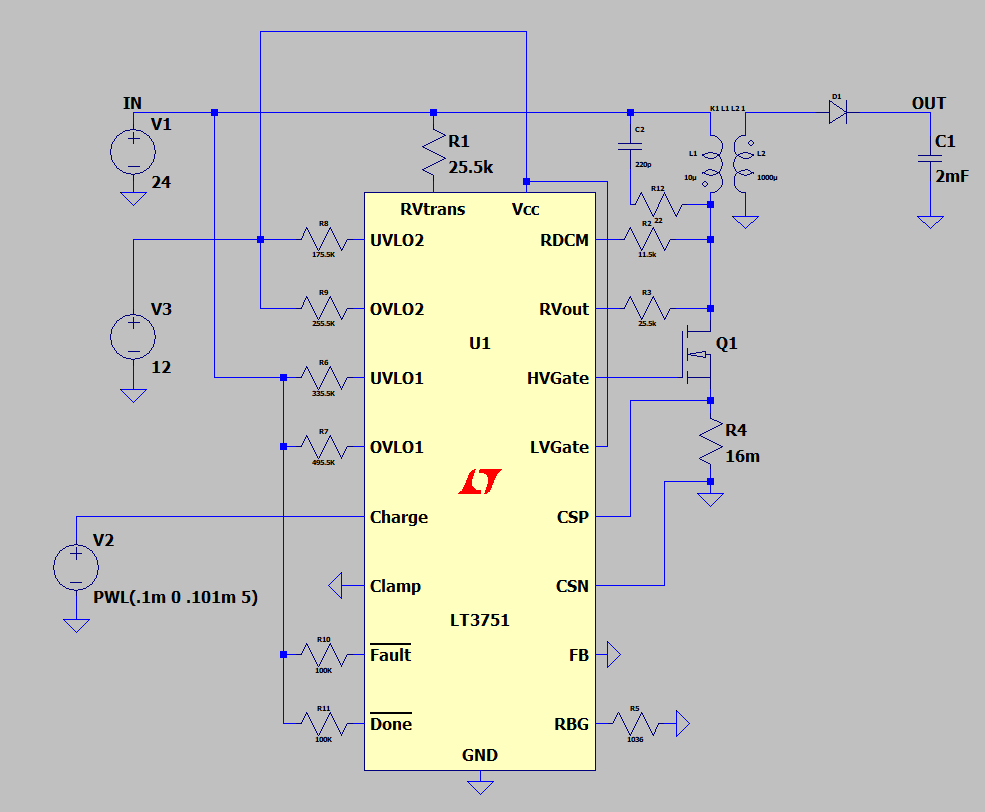
\includegraphics[width=\linewidth]{LT3571_Tbots_Configuration.png}
	\end{figure}
	
	\noindent The following variables were selected as design parameters:
	
	\begin{table}[h]
		\centering
		\begin{tabular}{lll}
			\textbf{Parameter}   & \textbf{Description}                      & \textbf{Value} \\
			\hline
			$V_{trans}$ & Transformer supply voltage       & 24V   \\
			$V_{out}$   & Output voltage                   & 240V  \\
			$C_{out}$   & Output capacitance               & 2mF   \\
			$I_{pk}$    & Peak transformer primary current & 10A  \\
			$VCC$		& Supply Voltage				   & 12V
		\end{tabular}
		\centering
	\end{table}
	
	\section{Pins}
	This section will briefly describe each pin and the calculations of any necessary components.\\
	
	\noindent \textbf{Note: Resistor values are calculated values and need to be updated with standard resistor values}
	
	\subsection{RVtrans}
	RVtrans is used as the transformer supply sense pin. The resistor $R_{trans}$ is placed between $V_{trans}$ and the pin. See Section 2 for instructions on setting $RV_{trans}$.
	
	\subsection{UVLO1, OVLO1, UVLO2, OVLO2}
	These four pins serve similar purposes, so they will be covered in the same section. UVLO1 and OVLO1 are the $V_{trans}$ undervoltage/overvoltage detection pins and will raise a fault signal when $V_{trans}$ drops below 18V or goes above 26V. They are connected to $V_{trans}$ via $R_{UVLO1}$ and $R_{OVLO1}$, which are calculated as per page 7 of the data sheet:
	\[R_{UVLO1} = \dfrac{V_{UVLO1} - 1.225V}{50\mu A} = \dfrac{18V - 1.225V}{50\mu A} = 335.5k\Omega\]
	\[R_{OVLO1} = \dfrac{V_{OVLO1} - 1.225V}{50\mu A} = \dfrac{26V - 1.225V}{50\mu A} = 495.5k\Omega\]
	UVLO2 and OVLO2 are the VCC undervoltage/overvoltage detection pins and will raise a fault signal when $VCC$ drops below 10V or goes above 14V. They are connected to $VCC$ via $R_{UVLO2}$ and $R_{OVLO2}$ which are calculated as follows:
	\[R_{UVLO2} = \dfrac{V_{UVLO2} - 1.225V}{50\mu A} = \dfrac{10V - 1.225V}{50\mu A} = 175.5k\Omega\]
	\[R_{OVLO2} = \dfrac{V_{OVLO2} - 1.225V}{50\mu A} = \dfrac{14V - 1.225V}{50\mu A} = 255.5k\Omega\]
	
	\subsection{Fault}
	This (active low) pin goes low when an undervoltage or overvoltage condition occurs and all switching will be disabled. The charge pin must be toggled to reset this signal. This pin must be pulled up to $V_{trans}$ or $VCC$ via a 100k$\Omega$ resistor.
	
	\subsection{Done}
	This (active low) pin goes low when the target output voltage is reached or the fault pin goes low. The charge pin must be toggled to reset this signal. This pin must be pulled up to $V_{trans}$ or $VCC$ via a 100k$\Omega$ resistor.
	
	\subsection{Charge}
	Drive pin higher than 1.5V to start charging. Bring to below 0.3V to stop charging. This pin is directly controlled by the microcontroller.
	
	\subsection{Clamp}
	Clamps the gate driver pin voltage. Clamp is set to 5.6V if this pin is connected to $VCC$ and 10.5V if connected to ground. In our implementation, $V_{GS}$ of our NMOS transistor is 10V so Clamp is connected to GND.
	
	\subsection{FB}
	Feedback regulation pin. The voltage of this pin determines whether the LT3571 is used as a no-load voltage regulator, heavy load voltage regulator, or capacitor charger. We connect this pin to ground for capacitor charger mode.
	
	\subsection{CSN and CSP}
	Negative and positive NMOS source current sense pins. Connect CSP to the source of the external transistor and CSN to ground, then connect a source resistor between CSP and CSN to complete the circuit. The value of this sense resistor is important as it sets the maximum value of the source current through the transistor, which by extension is the current through the transformer primary ($I_{pk}$). This resistor is calculated as follows:
	\[R_{CS} = \dfrac{106mV}{I_{pk}} = \dfrac{106mV}{10A} = 16m\Omega\]
	
	\subsection{VCC}
	12V input from the voltage regulator. Bypass with a XR5 ceramic cap because the data sheet says so.
	
	\subsection{LVGate}
	Low voltage gate pin. If $VCC$ is less than 8V, connect to external transistor gate. Otherwise connect to $VCC$. Our $VCC$ is 12V so this pin is connected to $VCC$. 
	
	\subsection{HVGate}
	High voltage gate pin. Connect to external transistor gate. Will drive gate voltage to within $VCC$-2V. Gets clamped based on the state of the Clamp pin.
	
	\subsection{RBG}
	This pin is really important because it sets the output voltage! Connect to ground via the $R_{BG}$ resistor. See section 2 for instructions on setting this resistor value.
	
	\subsection{RVout}
	Output voltage sense pin. Pretty self-explanatory. Connect to the external NMOS drain via the $R_{out}$ resistor. See section 2 for instructions on setting this resistor value.
	
	\subsection{RDCM}
	Discontinuous mode sense pin. Determines when to initiate the next switch cycle. Connect to the external NMOS drain via the $R_{DCM}$ resistor. See section 2 for instructions on setting this resistor value.
	
	\subsection{GND}
	Don't worry about it.
	
	\section{External Resistors}
	\subsection{RTrans, Rout, and RDCM}
	The values of $R_{trans}, R_{out}, \text{and } R_{DCM}$ are set based on $V_{trans}$ and $\Delta V_{Drain}$, where $\Delta V_{Drain}$ is the difference between $V_{Drain}$ (the drain of the external NMOS) and $V_{trans}$. $V_{Drain}$ is just $V_{out}$ + $V_{out}$ reflected back over the primary. 
	\[V_{Drain} = V_{trans} + \dfrac{V_{out}}{n} = 24V + \dfrac{240V}{10} = 48V\]
	We use this value for $\Delta V_{Drain}$:
	\[\Delta V_{Drain} = V_{Drain} - V_{trans} = 48V - 24V = 24V\]
	and compare it to Table 2 in the data sheet (pg 17):
	
	\begin{figure}[h!]
		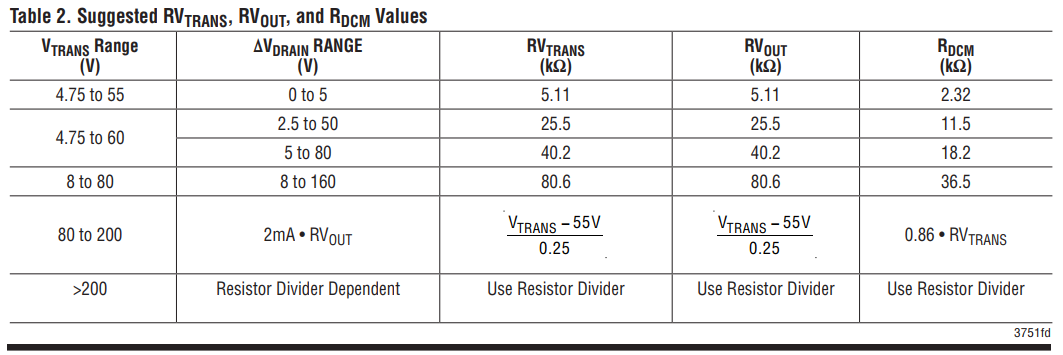
\includegraphics[width=\linewidth]{LT3571_Resistor_Values.png}
	\end{figure}

	\noindent Based on the table, $R_{trans} = 25.5k\Omega, R_{out} = 25.5k\Omega, \text{and } R_{DCM} = 11.5k\Omega$. These are also the values RoboJackets use so that's probably a good sign.

	\subsection{RBG}
	With the other resistors selected, $R_{BG}$ is calculated as follows (as per pg 45 of the data sheet):
	\[R_{BG} = 0.98N\dfrac{RV_{out}}{V_{out} + V_{diode}} = 0.98(10)\dfrac{25.5k\Omega}{240V + 1.7V} = 1033.9\Omega\]
	Where N is based on the flyback transformer (section 3.1) and $V_{diode}$ is the forward voltage of the output diode (section 3.2).
	
	\section{External Components}
	\subsection{Flyback Transformer}
	$I_{pk}$ is the main criteria for selecting the transformer. The CoilCraft DA-2034-AL is one of the transformers recommended by the LT3751 manufacturers (table 1 of the data sheet). It is the current frontrunner because of its ability to handle up to 10A on the primary, 1:10 ratio, and relatively small size. \textbf{Not available on digikey though (is available on Mouser).} This transformer is currently used by RoboJackets, while the similar CoilCraft DA-2032-AL is used by Mannheim ($I_{pk} = 5A$ for this transformer).
	\subsection{Output Diode}
	The output diode is selected based on the maximum repetitive reverse voltage ($V_{RRM}$) and the average forward current $I_{Av}$. The diode must meet the following requirements:
	\[V_{RRM} > V_{out} + N*V_{trans} = 240V + 10(24V)  = 480V\]
	\[I_{Av} > \dfrac{I_pk}{2N} = \dfrac{10A}{2*20} = 0.5A\]  
	The Fairchild ES3J is one of the diodes recommended by the LT3751 manufacturers (table 4 in the data sheet). It meets our requirements and has a low $t_{rr}$.
	\subsection{External NMOS}
	The Fairchild FDS2582 is one of the transistors recommended by the LT3751 manufacturers (table 3 in the data sheet).
	\subsection{RC Snubber Circuit}
	The purpose of the RC snubber circuit is to reduce the effect of the transformer leakage inductance. The transformer is not ideal; not all energy will be transferred from one coil to the other. When the MOSFET turns off, this energy needs to go somewhere. Otherwise, we will have a large voltage spike on the drain of the MOSFET, which may be enough to damage it. The voltage spike could also be enough for the comparator to think the capacitor bank is done charging, even if it's actually nowwhere near the charge voltage.\\\\
	Simulating the LT3751 with the non-ideal transformer was challenging, where seemingly impossible voltage spikes were noticed. After talking with Will from RoboJackets, I think that the spice model for the LT3751 is simply not designed to model a non-ideal transformer. Additionally, this simulation (and possibly the LT3751 itself) is incompatible with industry standard RCD or Zener snubber circuits.\\\\ 
	For the time being, our approach is to leave footprints for the RC snubber on the PCB and populate as needed. Will said that the transformer leakage inductance was small compared to the inductances caused by the high currents, and they were able to test different combinations of R and C in the snubber. We will use the same approach for the time being. 
\end{document}